% 真实照片取自开放获取论文；非本团队拍摄，非本模型实测验证。
% 完整出处、原出版PDF与SHA256见review/photo_sources.json及review/photo_archive。
\subsection{现场对象与负荷参数获取}
围护结构及使用条件影响建筑热损系数与得热。图\ref{fig:real-site-context}引用新疆大学研究人员在乌鲁木齐开展既有建筑改造研究时的建筑和热流计实拍\supcite{33}，说明建筑调查与热工测量对应的现场对象。这组照片作为参数获取的背景资料，原研究建筑与本文算例对象分别处理。

\begin{figure}[htbp]
\centering
\begin{minipage}[t]{0.46\textwidth}
\centering
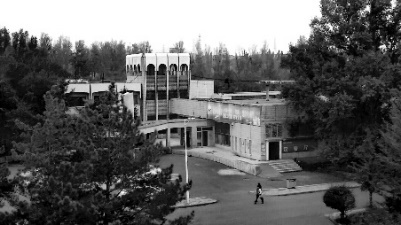
\includegraphics[height=38mm,width=\linewidth,keepaspectratio]{media/site_photos/urumqi_hotel_building.png}
\par\small （a）乌鲁木齐南郊既有旅馆
\end{minipage}\hfill
\begin{minipage}[t]{0.46\textwidth}
\centering
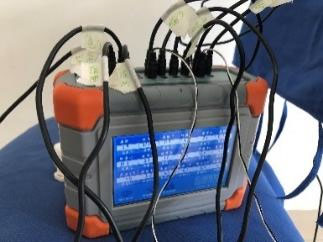
\includegraphics[height=38mm,width=\linewidth,keepaspectratio]{media/site_photos/urumqi_hotel_heat_flux_measurement.jpeg}
\par\small （b）原研究现场使用的多通道热流计
\end{minipage}
\caption{乌鲁木齐既有建筑与热流测量现场。取自Liao等\supcite{33}原图1左、图5左，CC BY 4.0；提取单幅照片并等比例排版，未修改照片内容。}
\label{fig:real-site-context}
\end{figure}
